\chapter{Baza danych}
\section{Wybór (Magdalena Solecka)}
\par Przy wyborze systemu do zarządzania bazą danych były brane pod uwagę \textit{Neo4j}\cite{Neo4j} oraz \textit{PostgreSQL}\cite{PostgreSQL}. Pierwsza z wymienionych wzbudziła zainteresowanie ze względu na planowaną implementację algorytmu rekomendującego Collaborative Filtering. Jej zaletą, jako grafowej bazy danych, byłoby szybkie wydobycie podobieństw pomiędzy użytkownikami na podstawie ocenionych przez nich miejsc. Uznano jednak, że zespół pracował do tej pory z relacyjnymi bazami danych i językiem SQL a dłuższe wykonanie algorytmu nie spowoduje problemów z wydajnym działaniem pozostałych funkcjonalności aplikacji, dlatego ostatecznie zdecydowano się na \textit{PostgreSQL} chwalonego za wysoką wydajność, oferującego wsparcie typu BJSON, który mógłby być przydatny przy  przechowywaniu większej ilości informacji o obiektach, a także znajomą zespołowi składnię zapytań. Bazę danych wdrożono w serwisie \textit{ElephantSQL} z instancją \textit{tiny turtle}
 która pozwalała na zapis 20 MB danych, 5 równoległych połączeń z bazą co było w zupełności wystarczające dla środowiska testowego.

\section{Schemat ERD (Magdalena Solecka)}
\par Zaprojektowany przy użyciu narzędzia \textit{ERD Constructor}.

\noindent\newline
\begin{figure}[h]
\centering
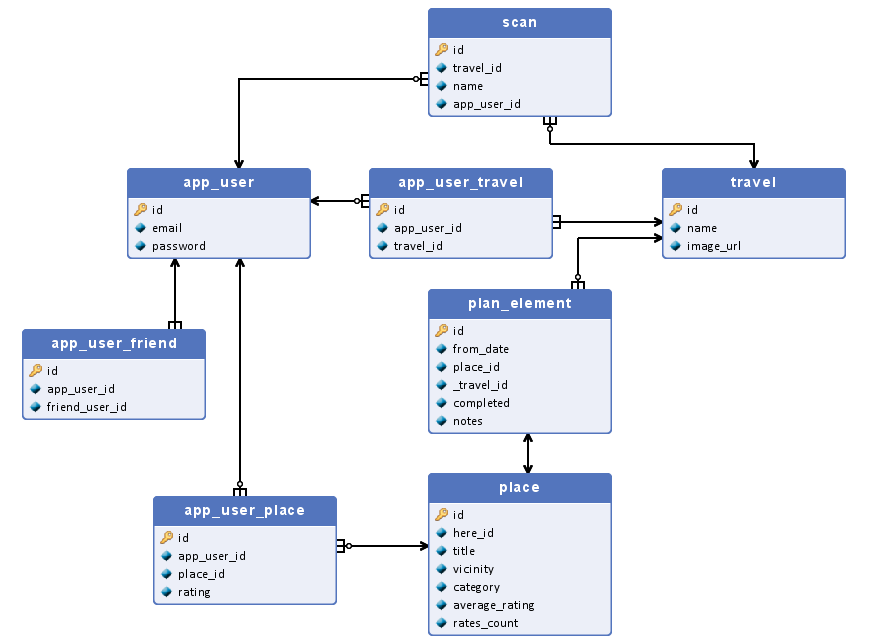
\includegraphics[width=\linewidth]{erd}
\caption{Diagram ERD}
\label{fig:erd}
\end{figure}
\FloatBarrier

\section{Praca z bazą danych (Magdalena Solecka)}
\par Warstwę danych tworzono podejściem \textit{najpierw kod} (ang. code first), głównie z powodu trudności z przewidzeniem, które struktury dostarczane przez zewnętrzne API uda się otrzymać i które informacje są niezbędne, aby znacząco nie zmniejszyć szybkości aplikacji, a o które można zapytać źródło podczas ładowania elementów ekranu. Stwarzało to problemy z kompatybilnością wsteczną podczas rozwijania aplikacji, dodawania nowych kolumn, zmiany typów. Początkowe rozwiązanie wymagało powiadomienia wszystkich programistów w zespole o godzinach, w których baza danych może przestać działać poprawnie, a przed jakąkolwiek dalsza pracą konieczne było ściągnięcie najnowszych zmian z repozytorium \textit{github}. Drugi w kolejności wprowadzonym sposobem było utworzenie tabeli tymczasowej -- wykonanie kopii tabeli oraz wprowadzenie zmian w kopii. Podmiany dokonywano przy dołączaniu zmian z gałęzi podrzędnej do gałęzi develop w serwisie \textit{github}. Nadal jednak wymagane było pobranie najnowszej wersji kodu. Z początku wymagało to zaplanowania pracy w ten sposób, aby lokalny kod nadawał się do zapisu (ang. commit) w chwili zmian w bazie, ale problem zakończył się odkryciem funkcji \textit{stash / unstash changes} oferowanej przez system \textit{Git}.
